\chapter{Introduction}
\label{ch:Introduction}
\acresetall

Optomechanics is the study of light-matter interactions; it is the study of how the intangible (light) can affect change in the tangible (matter) and vice versa. Injecting light into a material under specific conditions allows for an exchange of energy to occur between the light and the mechanical oscillations of the material which leaves the mechanical energy of the material altered. This interaction can be controlled to deposit or withdraw mechanical energy into/from a system and thus leave the system in a more, or less, mechanically energetic state respectively. The same interaction can also be harnessed for passive observation of material properties. Mechanical systems from bulk to atomic scales can be probed and characterized by light through retrieval of the inelastically scattered light resulting from interaction with the material. This retrieved light contains embedded information about the energy exchange that occurred, which, when considered as part of a population of scattering events, reveals the natural resonances and dissipation rates of mechanical modes.

Optomechanics comprises a broad range of phenomena involving the interaction of optical and mechanical systems, from basic photothermal absorption to more complex nonlinear processes. This section offers a brief overview of notable optomechanical phenomena. Photothermal absorption is the process by which light is absorbed by a material, leading to an increase in temperature of the material and consequent changes in the material's dimensions (thermal expansion) or refractive index (thermo-optic effect). This effect has applications in optical switches, actuators, and sensors. \cite{boccara1980thermo, sutar2024design} Photothermal therapy in medicine is an emerging application of this effect, where light is used to target and heat specific areas, causing localized damage to diseased tissue\cite{hirsch2003nanoshell}. This technique becomes especially effective when combined with nanoparticle-enhanced absorption, allowing for dramatically increased absorption in ultra-localized zones within the body. \cite{johnson2018hybridization}

Light scattering, in its many forms, is also an optomechanical process as it involves the interaction of an optical field with the fluctuation, motion, or vibration of matter. Rayleigh scattering, perhaps the most well-known example, is the elastic scattering of light by particles much smaller than the wavelength of the incident light, leading to scattering in possibly a new direction but without a change in wavelength. It is responsible for the blue color of the sky because the efficiency of Rayleigh scattering is inversely proportional to the fourth power of the wavelength (\(\lambda\)) of the light (\(\frac{1}{\lambda^{4}}\)) and so shorter (blue) wavelengths are scattered much more than longer (red) wavelengths by the molecules in the atmosphere.\cite{rayleigh1871light}

Raman scattering is the interaction of light with vibrational and rotational modes within a material (often molecular), resulting in scattered light with frequencies that are shifted from the incident light. This inelastically scattered light provides insights into the material's molecular structure and properties. Raman scattering is widely used in chemical and material science for identifying chemical compounds, analyzing molecular structures, and studying molecular dynamics. It finds application in the characterization of pharmaceuticals, monitoring changes in biological tissues for medical diagnostics, and investigation of stress and temperature distributions in engineering materials, among others. \cite{vankeirsbilck2002applications, krafft2015many}

Brillouin scattering, around which much of the work detailed in this document is centered, is the scattering of light with acoustic phonons or coherent traveling density waves in a material, resulting in scattered light with a frequency that is slightly shifted from the incident light. This inelastically scattered light reveals mechanical properties of the material such as its bulk and elastic moduli. This phenomenon is used in materials science to measure elastic properties and viscoelasticity of materials, in fiber optic sensing to monitor temperature and strain over large distances, and in physics to study phase transitions and mechanical properties of crystals, liquids, and gases. \cite{scarcelli2008confocal, horiguchi1990technique, brody1968brillouin}

Rayleigh-wing scattering is the broad, smooth extension of the Rayleigh scattering spectrum that results from interactions with low-frequency excitations in a material, providing insights into dynamic processes like rotational and translational diffusion of molecules that make up a material. This scattering is particularly useful in studying the dynamics of complex fluids, gases, and soft materials, where it can reveal information about molecular orientation, diffusion rates, and interactions within the medium. Applications include the analysis of atmospheric phenomena, characterization of liquid crystals, and investigations into the properties of polymers and biological materials, aiding in the understanding of their behavior at the molecular level. \cite{bodhaine1999rayleigh, amer1975temperature}

Figure \ref{fig:Introduction:scattering-domains} shows the relative domains of typical frequency shifts for Rayleigh, Rayleigh-wing, Brillouin, and Raman scattering. Rayleigh-wing scattering is broad and shares part of its domain with Brillouin scattering. This makes sense because for any given molecule and within the timescale that it occurs, diffusive translational motion can be thought of as indistinguishable from motion caused by traveling density waves that host brillouin scattering. In this way, Rayleigh-wing scattering represents a sporadic distribution of fleeting, localized Brillouin scattering. Of course, the difference between incoherent diffusion of molecules and coherently traveling acoustic modes within a material is an important distinction. However, this thought experiment offers a perspective for bridging the gap between Rayleigh-wing and Brillouin scattering and for understanding their common frequency domains. Moreover, it serves as a reminder of the rich continuum of material behavior and responses that affect light scattering as opposed to the distinct categories we ascribe for convenience. This is a core concept of the research described in further chapters.%Boyd 9.6 works out general theory of Brillouin and Rayleigh scattering!

% This makes sense, as the [random and incoherent] translational motion of molecules as they [continuously] diffuse [according to the laws of thermodynamics and as described by statistical mechanics] can be thought of, within the timescale that this motion occurs, as indistinguishable from [translational motion as caused by coherent] traveling density waves which host brillouin scattering.

\begin{figure}[t] % here (h), at the top (t), at the bottom (b), or on a separate page for floats (p), in that preference order
\centering
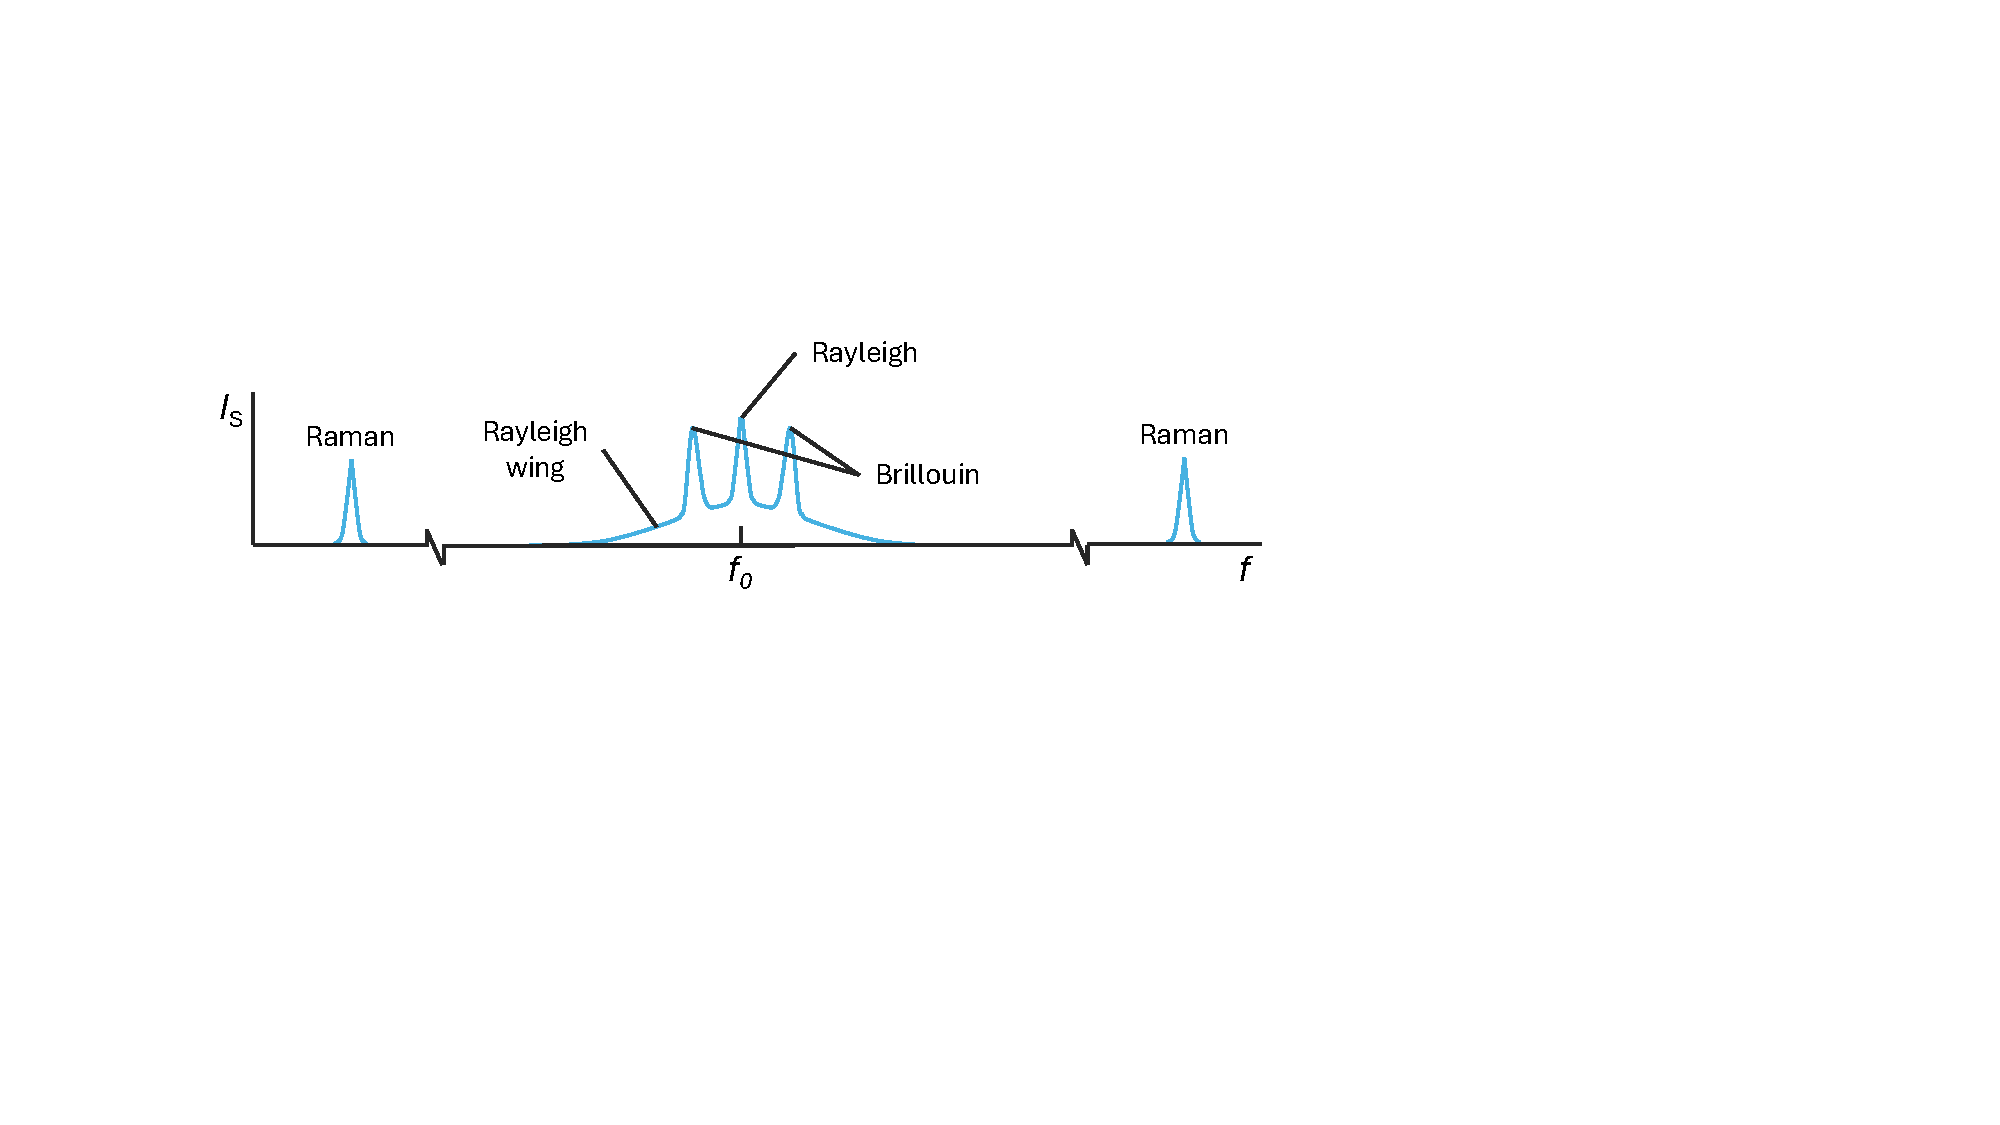
\includegraphics[width=\textwidth]{figs/1-Intro/frequencyShifts.pdf}
\caption[Relative domains of typical frequency shifts for Rayleigh, Rayleigh-wing, Brillouin, and Raman scattering.]{Relative domains of typical frequency shifts for Rayleigh, Rayleigh-wing, Brillouin, and Raman scattering. Figure adapted from Boyd Nonlinear Optics (2020). \cite{boyd2020nonlinear}}
\label{fig:Introduction:scattering-domains}
\end{figure}

Returning to other optomechanical phenomena beyond scattering processes, the momentum of photons can exert forces on objects, leading to phenomena like radiation pressure, optical tweezing, and optical trapping. These effects are widely used in manipulating microscopic particles, biological cells, and atoms, enabling studies of single molecules, cold atoms, and quantum computing elements. \cite{ashkin1987optical, raab1987trapping, browaeys2020many}

The final category of optomechanical interactions to be noted here is that of nonlinear optical phenomena. Second harmonic generation, parametric oscillation, and four-wave mixing all feature the interaction between light and material nonlinearities that lead to the generation of new light frequencies.\cite{boyd2020nonlinear} The Kerr effect is the change in the refractive index of a material in response to an applied electric field, which can be induced optically with sufficient intensities of light. In general, nonlinear optical responses of materials are often only accessible with the use of high intensity laser light. This is emphasized by the fact that the field of nonlinear optics can be traced back to the discovery of second-harmonic generation in 1961\cite{franken1961generation}, just one year after the first demonstration of the laser by American physicist Theodor Maiman.\cite{maiman1960stimulated} These nonlinear effects provide the foundation for a range of technologies, including high-speed optical communication systems, frequency converters, and lasers for materials processing. \cite{franken1961generation, mollenauer1980experimental, strickland1985compression} Also included in nonlinear optical phenomena is electrostriction. Electrostriction is a reversible material deformation induced by an electric field, which can be generated by light in electro-optic materials. This effect is quadratic, scaling with the square of the applied electric field, and hence a nonlinear optical effect. At sufficiently high intensities, electrostrictive forces serve to enhance Brillouin scattering whereby the scattered light electrostrictively reinforces the acoustic wave that caused its scattering, leading to a nonlinear positive feedback loop known as \ac{SBS}. Photostriction is a related phenomenon that occurs when light absorption causes a change in the lattice structure of a material, leading to mechanical strain. It combines photovoltaic and piezoelectric effects and can be seen as optically induced strain. These effects are utilized in designing optical modulators, tunable photonic devices, and smart materials that respond to light. \cite{haertling1971hot, chu1995photostrictive}


This dissertation is organized into three core chapters, each centered on harnessing traveling-wave phonon dynamics through Brillouin scattering. Chapter~\ref{ch:Cooling} presents the first experimental demonstration of laser cooling of a continuum of traveling acoustic phonons in a macroscopic medium via anti-Stokes Brillouin scattering. By leveraging the strong acousto-optic coupling in a liquid fiber core, we observe a power-dependent suppression of thermal phonons corresponding to a \(>\)\SI{20}{\kelvin} reduction of the acoustic mode’s effective temperature. This result extends the paradigm of continuous-mode optomechanical cooling, previously only achieved in chip-scale waveguides, to a meter-scale fiber system, highlighting the universality and scalability of traveling-wave phonon manipulation. Chapter~\ref{ch:CoBS} introduces an ultra-sensitive four-wave-mixing phonon spectrometer (\acs{CoBS}), which we developed to probe Brillouin interactions with unprecedented sensitivity. The \ac{CoBS} instrument uses coherent pump–probe stimulation to amplify phonon signals, achieving \si{\femto\watt} detection limits that enable Brillouin scattering measurements in extremely short interaction lengths. Producing \(\sim\)\(10^{6}\) more scattered power than conventional Brillouin scattering techniques, this advanced methodology provides a new window into phonon spectra and dynamics, laying the experimental groundwork for observing extremely subtle phononic phenomena. Chapter~\ref{ch:Raman} explores the emergence of Raman-like phonon modes induced by traveling-wave Brillouin interactions across a range of material platforms. By systematically shrinking the acoustic path length (from meters to sub-millimeter scales) and enhancing phonon reflectivity in media including doped optical fibers, bulk liquids, thin films of tellurium dioxide, and integrated waveguides, we probe the crossover between the continuous Brillouin regime and discrete standing-wave vibrational modes. These experiments approach the regime in which traveling acoustic waves “freeze” into bounded modes; where traveling-wave Brillouin scattering morphs into Raman-like phonon resonances. This pursuit effectively unifies the Brillouin (traveling-wave) and Raman (standing-wave) paradigms of light–sound interaction, providing new opportunities in cavity-free phononics and coherent phonon devices at room temperature. Taken together, the work and results presented here underscore traveling-wave Brillouin scattering as a versatile tool for phonon manipulation, from optical cooling of phonon populations to high-precision phonon spectroscopy and the generation of novel phononic modes at room temperature. Brillouin-mediated light–sound coupling enables these diverse advances and links them to the broader context of hybrid photonic–phononic technologies. By demonstrating control over traveling phonons in continuous media, developing instrumentation to detect minute phonon signals, and pushing toward the Brillouin–Raman convergence, this work contributes to emerging frontiers in both classical and quantum acoustics. In particular, this work suggests new avenues for acousto-optic devices with reduced noise (through phonon cooling) and lay groundwork for quantum acoustic control in room-temperature systems. The subsequent chapters detail these contributions, collectively advancing the goal of manipulating sound waves with light in unprecedented ways.


%The remainder of this chapter further describes the specific optomechanical phenomena that pertain to the research presented in this document: Brillouin scattering, electrostriction as it pertains to the \ac{SBS} process, and Raman scattering.

%--------------------------------------------------------------------%

% \section{Light Scattering}
% \label{Introduction:sec:LightScattering}
% Light scattering involves the redirection of light as a result of interactions with the constituent particles or molecules within a material medium. In every case, light scattering occurs because of variations in the material's optical properties. To understand why, envision a material with completely uniform particles---spatially and temporally consistent, or in other words, perfectly homogeneous. Figure \ref{fig:Introduction:homogeneous-material-no-scatter} shows an incident optical plane wave encountering a segment of such a material, denoted $\delta z$, containing a volume element $\delta V_{1}$. For any given incident wavelength $\lambda$ and any non-zero scattering angle $\theta$ at volume $\delta V_{1}$, there exists a corresponding volume element $\delta V_{2}$, located a distance $\frac{\lambda}{2\sin\theta}$ apart, which scatters light at the same angle $\theta$. The scattered waves from $\delta V_{1}$ and $\delta V_{2}$ would be out of phase by $\frac{\lambda}{2}$, leading to perfect destructive interference and no resultant scattered field. Thus, to achieve observable scattering, the material must possess inhomogeneities, allowing for variations in the optical properties between neighboring volumes. Fortunately, perfect homogeneity is not characteristic of real materials; all matter undergoes thermodynamic fluctuations at any temperature above absolute zero, and quantum fluctuations are inherent even at the ground state.

%We now begin with a theoretical description of spontaneous light scattering as a result of thermodynamic fluctuations, presented in Boyd Nonlinear Optics.\cite{boyd2020nonlinear} This foundation will serve as a framework for distinguishing between light that scatters as a result of coherent propagating pressure or density variations (Brillouin scattering) and light that scatters as a result of static or random thermodynamic variations (Rayleigh scattering). Later we will treat the case of higher-intensity \ac{SBS}. Ultimately we will build upon this theoretical basis to derive the coupled-wave equations of \ac{CoBS}, a novel instrument which underpins many of the results presented in future chapters. To begin building a theoretical description of light scattering, we consider thermodynamic fluctuations as the origin of the scattering process.

%Maxwell's equations -> scattering from Zangwill?

%Boyd 8.3

% \begin{figure}[t] % here (h), at the top (t), at the bottom (b), or on a separate page for floats (p), in that preference order
% \centering
% 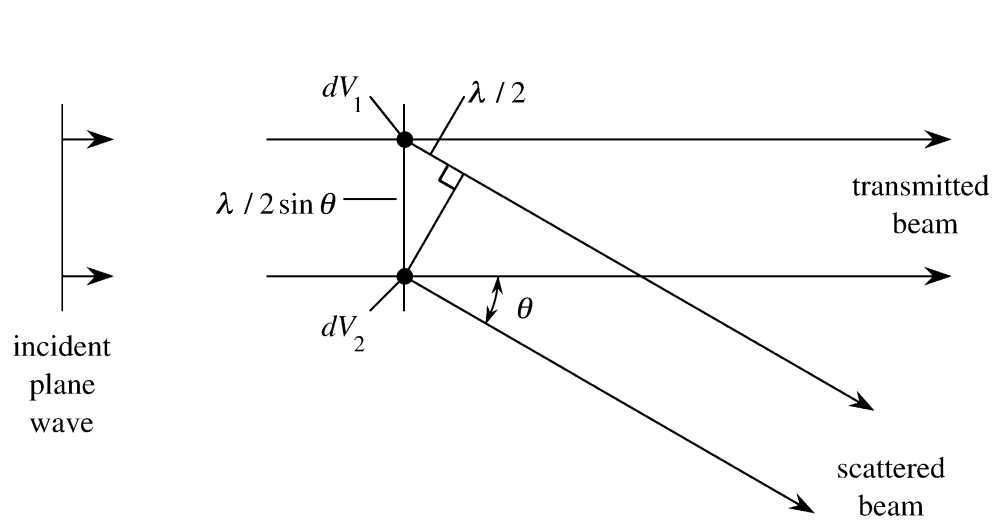
\includegraphics[width=\textwidth]{figs/1-Intro/Boyd homogeneous material no scatter.png}
% \caption{}
% \label{fig:Introduction:homogeneous-material-no-scatter}
% \end{figure}

% \section{Spontaneous Brillouin Scattering}
% \label{sec:Introduction:Spontaneous-Brillouin}
%
%
% \section{Stimulated Brillouin Scattering}
% \label{sec:Introduction:Stimulated}
%
%
% \section{Phase-matching}
% \label{sec:Introduction:Phase-matching}
%
%
% \section{Brillouin Gain of Materials}
% \label{subsec:Introduction:Gain}
%
%
% \section{Raman Scattering}
% \label{sec:Introduction:Raman}
%
%
% \section{Raman-like Brillouin Modes}
% \label{sec:Introduction:Raman-like}


\clearpage
\thispagestyle{empty}
\null
\newpage
